\documentclass[twoside]{book}

% Packages required by doxygen
\usepackage{fixltx2e}
\usepackage{calc}
\usepackage{doxygen}
\usepackage[export]{adjustbox} % also loads graphicx
\usepackage{graphicx}
\usepackage[utf8]{inputenc}
\usepackage{makeidx}
\usepackage{multicol}
\usepackage{multirow}
\PassOptionsToPackage{warn}{textcomp}
\usepackage{textcomp}
\usepackage[nointegrals]{wasysym}
\usepackage[table]{xcolor}

% Font selection
\usepackage[T1]{fontenc}
\usepackage[scaled=.90]{helvet}
\usepackage{courier}
\usepackage{amssymb}
\usepackage{sectsty}
\renewcommand{\familydefault}{\sfdefault}
\allsectionsfont{%
  \fontseries{bc}\selectfont%
  \color{darkgray}%
}
\renewcommand{\DoxyLabelFont}{%
  \fontseries{bc}\selectfont%
  \color{darkgray}%
}
\newcommand{\+}{\discretionary{\mbox{\scriptsize$\hookleftarrow$}}{}{}}

% Page & text layout
\usepackage{geometry}
\geometry{%
  a4paper,%
  top=2.5cm,%
  bottom=2.5cm,%
  left=2.5cm,%
  right=2.5cm%
}
\tolerance=750
\hfuzz=15pt
\hbadness=750
\setlength{\emergencystretch}{15pt}
\setlength{\parindent}{0cm}
\setlength{\parskip}{3ex plus 2ex minus 2ex}
\makeatletter
\renewcommand{\paragraph}{%
  \@startsection{paragraph}{4}{0ex}{-1.0ex}{1.0ex}{%
    \normalfont\normalsize\bfseries\SS@parafont%
  }%
}
\renewcommand{\subparagraph}{%
  \@startsection{subparagraph}{5}{0ex}{-1.0ex}{1.0ex}{%
    \normalfont\normalsize\bfseries\SS@subparafont%
  }%
}
\makeatother

% Headers & footers
\usepackage{fancyhdr}
\pagestyle{fancyplain}
\fancyhead[LE]{\fancyplain{}{\bfseries\thepage}}
\fancyhead[CE]{\fancyplain{}{}}
\fancyhead[RE]{\fancyplain{}{\bfseries\leftmark}}
\fancyhead[LO]{\fancyplain{}{\bfseries\rightmark}}
\fancyhead[CO]{\fancyplain{}{}}
\fancyhead[RO]{\fancyplain{}{\bfseries\thepage}}
\fancyfoot[LE]{\fancyplain{}{}}
\fancyfoot[CE]{\fancyplain{}{}}
\fancyfoot[RE]{\fancyplain{}{\bfseries\scriptsize Generated by Doxygen }}
\fancyfoot[LO]{\fancyplain{}{\bfseries\scriptsize Generated by Doxygen }}
\fancyfoot[CO]{\fancyplain{}{}}
\fancyfoot[RO]{\fancyplain{}{}}
\renewcommand{\footrulewidth}{0.4pt}
\renewcommand{\chaptermark}[1]{%
  \markboth{#1}{}%
}
\renewcommand{\sectionmark}[1]{%
  \markright{\thesection\ #1}%
}

% Indices & bibliography
\usepackage{natbib}
\usepackage[titles]{tocloft}
\setcounter{tocdepth}{3}
\setcounter{secnumdepth}{5}
\makeindex

% Hyperlinks (required, but should be loaded last)
\usepackage{ifpdf}
\ifpdf
  \usepackage[pdftex,pagebackref=true]{hyperref}
\else
  \usepackage[ps2pdf,pagebackref=true]{hyperref}
\fi
\hypersetup{%
  colorlinks=true,%
  linkcolor=blue,%
  citecolor=blue,%
  unicode%
}

% Custom commands
\newcommand{\clearemptydoublepage}{%
  \newpage{\pagestyle{empty}\cleardoublepage}%
}

\usepackage{caption}
\captionsetup{labelsep=space,justification=centering,font={bf},singlelinecheck=off,skip=4pt,position=top}

%===== C O N T E N T S =====

\begin{document}

% Titlepage & ToC
\hypersetup{pageanchor=false,
             bookmarksnumbered=true,
             pdfencoding=unicode
            }
\pagenumbering{alph}
\begin{titlepage}
\vspace*{7cm}
\begin{center}%
{\Large My Project }\\
\vspace*{1cm}
{\large Generated by Doxygen 1.8.13}\\
\end{center}
\end{titlepage}
\clearemptydoublepage
\pagenumbering{roman}
\tableofcontents
\clearemptydoublepage
\pagenumbering{arabic}
\hypersetup{pageanchor=true}

%--- Begin generated contents ---
\chapter{Todo List}
\label{todo}
\Hypertarget{todo}

\begin{DoxyRefList}
\item[\label{todo__todo000002}%
\Hypertarget{todo__todo000002}%
Member \hyperlink{classAFMatrix_a918b5f7c03cb3a305ec94e08afd3e09a}{A\+F\+Matrix$<$ T $>$\+:\+:A\+F\+Matrix} (A\+F\+Matrix$<$ T $>$ $\ast$copy\+From)]Make this effecient and non-\/copying  
\item[\label{todo__todo000003}%
\Hypertarget{todo__todo000003}%
Member \hyperlink{classAFMatrix_a0dfd54218d171d086a738a0525c5946e}{A\+F\+Matrix$<$ T $>$\+:\+:A\+F\+Matrix} (int num\+Rows, int num\+Cols, vector$<$ T $>$ $\ast$copy\+From\+Array)]Make this effecient and non-\/copying  
\item[\label{todo__todo000004}%
\Hypertarget{todo__todo000004}%
Member \hyperlink{classAFMatrix_a63cc8c6b50d757fc75049a35a9123588}{A\+F\+Matrix$<$ T $>$\+:\+:copy\+Values} (A\+F\+Matrix$<$ T $>$ $\ast$dst, vector$<$ T $>$ $\ast$src)]Clarify how things work if matrices can be row-\/major or column-\/major.  
\item[\label{todo__todo000001}%
\Hypertarget{todo__todo000001}%
Member \hyperlink{classAFMatrix_a124e51921d4275e00354d3af98399d1e}{A\+F\+Matrix$<$ T $>$\+:\+:vals} ]Is vals dynamically allocated or what?? $\vert$ a b $\vert$~\newline
$\vert$ c d $\vert$ = \mbox{[}a b c d e f\mbox{]}~\newline
$\vert$ e f $\vert$~\newline

\end{DoxyRefList}
\chapter{Hierarchical Index}
\section{Class Hierarchy}
This inheritance list is sorted roughly, but not completely, alphabetically\+:\begin{DoxyCompactList}
\item \contentsline{section}{A\+F\+Activation\+Function}{\pageref{class_a_f_activation_function}}{}
\begin{DoxyCompactList}
\item \contentsline{section}{Re\+LU}{\pageref{class_re_l_u}}{}
\end{DoxyCompactList}
\item \contentsline{section}{A\+F\+Matrix$<$ T, R\+O\+WS, C\+O\+LS $>$}{\pageref{class_a_f_matrix}}{}
\item \contentsline{section}{A\+F\+Matrix$<$ double, L\+E\+N\+\_\+\+O\+UT, L\+E\+N\+\_\+\+IN $>$}{\pageref{class_a_f_matrix}}{}
\item \contentsline{section}{Layer$<$ L\+E\+N\+\_\+\+IN, L\+E\+N\+\_\+\+O\+UT $>$}{\pageref{class_layer}}{}
\item \contentsline{section}{Net$<$ T $>$}{\pageref{class_net}}{}
\end{DoxyCompactList}

\chapter{Class Index}
\section{Class List}
Here are the classes, structs, unions and interfaces with brief descriptions\+:\begin{DoxyCompactList}
\item\contentsline{section}{\hyperlink{class_a_f_activation_function}{A\+F\+Activation\+Function$<$ T, N, M $>$} }{\pageref{class_a_f_activation_function}}{}
\item\contentsline{section}{\hyperlink{class_a_f_loss_function}{A\+F\+Loss\+Function$<$ T, N, M $>$} }{\pageref{class_a_f_loss_function}}{}
\item\contentsline{section}{\hyperlink{class_a_f_matrix}{A\+F\+Matrix$<$ T, R\+O\+W\+S, C\+O\+L\+S $>$} }{\pageref{class_a_f_matrix}}{}
\item\contentsline{section}{\hyperlink{class_a_f_square_loss_function}{A\+F\+Square\+Loss\+Function$<$ T, N, M $>$} }{\pageref{class_a_f_square_loss_function}}{}
\item\contentsline{section}{\hyperlink{class_identity_function}{Identity\+Function$<$ T, N, M $>$} }{\pageref{class_identity_function}}{}
\item\contentsline{section}{\hyperlink{class_layer}{Layer$<$ L\+E\+N\+\_\+\+I\+N, L\+E\+N\+\_\+\+O\+U\+T $>$} }{\pageref{class_layer}}{}
\item\contentsline{section}{\hyperlink{class_net}{Net$<$ T $>$} }{\pageref{class_net}}{}
\item\contentsline{section}{\hyperlink{class_re_l_u}{Re\+L\+U$<$ T, N, M $>$} }{\pageref{class_re_l_u}}{}
\end{DoxyCompactList}

\chapter{File Index}
\section{File List}
Here is a list of all files with brief descriptions\+:\begin{DoxyCompactList}
\item\contentsline{section}{C\+:/\+Users/\+Aryan/\+C\+Lion\+Projects/\+C\+Net/src/\hyperlink{_a_f_activation_function_8cpp}{A\+F\+Activation\+Function.\+cpp} }{\pageref{_a_f_activation_function_8cpp}}{}
\item\contentsline{section}{C\+:/\+Users/\+Aryan/\+C\+Lion\+Projects/\+C\+Net/src/\hyperlink{_a_f_activation_function_8h}{A\+F\+Activation\+Function.\+h} }{\pageref{_a_f_activation_function_8h}}{}
\item\contentsline{section}{C\+:/\+Users/\+Aryan/\+C\+Lion\+Projects/\+C\+Net/src/\hyperlink{_a_f_matrix_8cpp}{A\+F\+Matrix.\+cpp} }{\pageref{_a_f_matrix_8cpp}}{}
\item\contentsline{section}{C\+:/\+Users/\+Aryan/\+C\+Lion\+Projects/\+C\+Net/src/\hyperlink{_a_f_matrix_8h}{A\+F\+Matrix.\+h} }{\pageref{_a_f_matrix_8h}}{}
\item\contentsline{section}{C\+:/\+Users/\+Aryan/\+C\+Lion\+Projects/\+C\+Net/src/\hyperlink{_layer_8cpp}{Layer.\+cpp} }{\pageref{_layer_8cpp}}{}
\item\contentsline{section}{C\+:/\+Users/\+Aryan/\+C\+Lion\+Projects/\+C\+Net/src/\hyperlink{_layer_8h}{Layer.\+h} }{\pageref{_layer_8h}}{}
\item\contentsline{section}{C\+:/\+Users/\+Aryan/\+C\+Lion\+Projects/\+C\+Net/src/\hyperlink{main_8cpp}{main.\+cpp} }{\pageref{main_8cpp}}{}
\item\contentsline{section}{C\+:/\+Users/\+Aryan/\+C\+Lion\+Projects/\+C\+Net/src/\hyperlink{_net_8cpp}{Net.\+cpp} }{\pageref{_net_8cpp}}{}
\item\contentsline{section}{C\+:/\+Users/\+Aryan/\+C\+Lion\+Projects/\+C\+Net/src/\hyperlink{_net_8h}{Net.\+h} }{\pageref{_net_8h}}{}
\end{DoxyCompactList}

\chapter{Class Documentation}
\hypertarget{class_a_f_activation_function}{}\section{A\+F\+Activation\+Function Class Reference}
\label{class_a_f_activation_function}\index{A\+F\+Activation\+Function@{A\+F\+Activation\+Function}}


{\ttfamily \#include $<$A\+F\+Activation\+Function.\+h$>$}

Inheritance diagram for A\+F\+Activation\+Function\+:\begin{figure}[H]
\begin{center}
\leavevmode
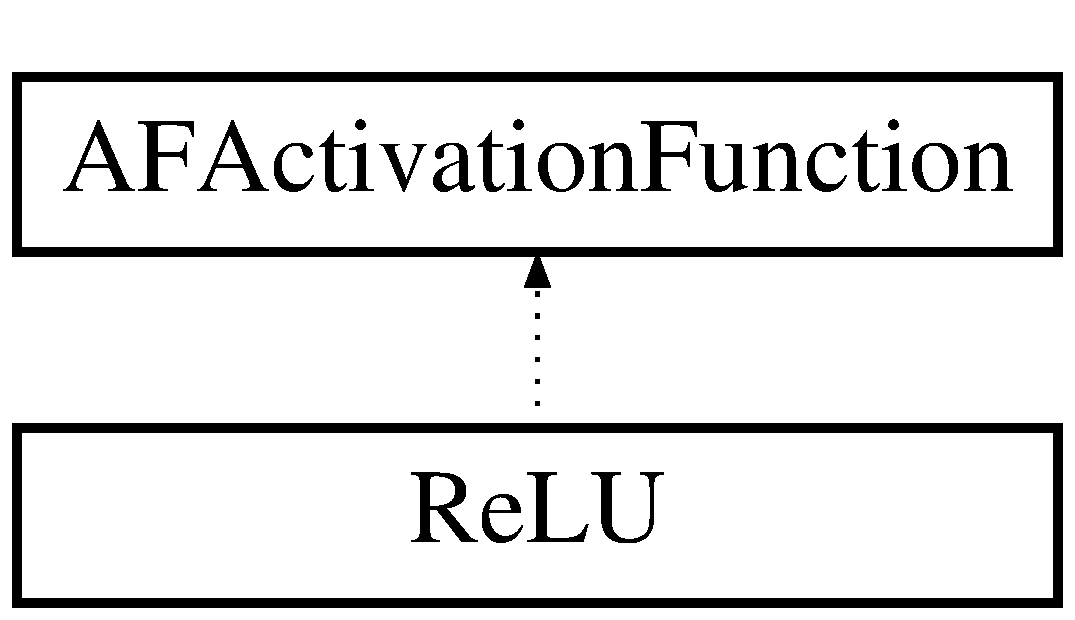
\includegraphics[height=2.000000cm]{class_a_f_activation_function}
\end{center}
\end{figure}


The documentation for this class was generated from the following file\+:\begin{DoxyCompactItemize}
\item 
C\+:/\+Users/\+Aryan/\+C\+Lion\+Projects/\+C\+Net/src/\hyperlink{_a_f_activation_function_8h}{A\+F\+Activation\+Function.\+h}\end{DoxyCompactItemize}

\hypertarget{class_a_f_matrix}{}\section{A\+F\+Matrix$<$ T, R\+O\+WS, C\+O\+LS $>$ Class Template Reference}
\label{class_a_f_matrix}\index{A\+F\+Matrix$<$ T, R\+O\+W\+S, C\+O\+L\+S $>$@{A\+F\+Matrix$<$ T, R\+O\+W\+S, C\+O\+L\+S $>$}}


{\ttfamily \#include $<$A\+F\+Matrix.\+h$>$}

\subsection*{Public Member Functions}
\begin{DoxyCompactItemize}
\item 
\hyperlink{class_a_f_matrix_a6ccd1bdad16dfa7ef38db5e0fc4e0e2b}{A\+F\+Matrix} ()
\item 
\hyperlink{class_a_f_matrix_ae76418eb02f3f9b84ee13aebaeca564a}{A\+F\+Matrix} (\hyperlink{class_a_f_matrix}{A\+F\+Matrix}$<$ T, R\+O\+WS, C\+O\+LS $>$ $\ast$copy\+From)
\item 
\hyperlink{class_a_f_matrix_adf63ea3dbdc05d678371099310993471}{A\+F\+Matrix} (array$<$ T, R\+O\+WS $\ast$C\+O\+LS $>$ $\ast$copy\+From)
\item 
\hyperlink{class_a_f_matrix_a657752979ec2d7bad591e3def1f4bcc7}{$\sim$\+A\+F\+Matrix} ()
\item 
T \hyperlink{class_a_f_matrix_a1363727b7a4b97bad5e7c9d9552d9cf5}{get\+Index} (int row, int col)
\item 
T \hyperlink{class_a_f_matrix_a0e36b5c6f333ac3d6508d5b00c92852c}{get\+Value} (int row, int col)
\item 
{\footnotesize template$<$size\+\_\+t O\+T\+H\+E\+R\+\_\+\+C\+O\+LS$>$ }\\void \hyperlink{class_a_f_matrix_a2c3183f964593d1bc52f6dc09429dbcc}{inner\+Product} (\hyperlink{class_a_f_matrix}{A\+F\+Matrix}$<$ T, C\+O\+LS, O\+T\+H\+E\+R\+\_\+\+C\+O\+LS $>$ $\ast$other, \hyperlink{class_a_f_matrix}{A\+F\+Matrix}$<$ T, R\+O\+WS, O\+T\+H\+E\+R\+\_\+\+C\+O\+LS $>$ $\ast$out)
\item 
void \hyperlink{class_a_f_matrix_a9f0e4b22b84400a30d275be6bd67d128}{inner\+Product} (array$<$ T, R\+O\+WS $>$ $\ast$other, \hyperlink{class_a_f_matrix}{A\+F\+Matrix}$<$ T, C\+O\+LS, 1 $>$ $\ast$out)
\item 
void \hyperlink{class_a_f_matrix_ad2763218bc42414ca32cdecba3b88be2}{inner\+Product} (array$<$ T, R\+O\+WS $>$ $\ast$other, array$<$ T, C\+O\+LS $>$ $\ast$out)
\item 
void \hyperlink{class_a_f_matrix_ae087fb4a064d256eac51513863b06fa2}{transpose} (\hyperlink{class_a_f_matrix}{A\+F\+Matrix}$<$ T, C\+O\+LS, R\+O\+WS $>$ $\ast$out)
\item 
\hyperlink{class_a_f_matrix}{A\+F\+Matrix} $\ast$ \hyperlink{class_a_f_matrix_a5f20b3ee2b16cbb9b9b39215a81d3aa1}{transpose} ()
\item 
void \hyperlink{class_a_f_matrix_a905b58769fceaf03972f7ea179ea3934}{scale} (double factor, \hyperlink{class_a_f_matrix}{A\+F\+Matrix} $\ast$out)
\item 
void \hyperlink{class_a_f_matrix_aad31e9f92bfa3323313b153fddcd676b}{add} (\hyperlink{class_a_f_matrix}{A\+F\+Matrix} $\ast$other, \hyperlink{class_a_f_matrix}{A\+F\+Matrix} $\ast$out)
\item 
void \hyperlink{class_a_f_matrix_a8826fb01197325729f0516721e14027f}{subtract} (\hyperlink{class_a_f_matrix}{A\+F\+Matrix} $\ast$other, \hyperlink{class_a_f_matrix}{A\+F\+Matrix} $\ast$out)
\item 
array$<$ T, R\+O\+WS $\ast$C\+O\+LS $>$ $\ast$ \hyperlink{class_a_f_matrix_a7e3659073ff6da5ffd02de48156decf5}{to\+Array} ()
\item 
void \hyperlink{class_a_f_matrix_ad44dc733a8bcf412437d0beebd458176}{copy\+Values} (\hyperlink{class_a_f_matrix}{A\+F\+Matrix}$<$ T, R\+O\+WS, C\+O\+LS $>$ $\ast$dst, \hyperlink{class_a_f_matrix}{A\+F\+Matrix}$<$ T, R\+O\+WS, C\+O\+LS $>$ $\ast$src)
\item 
void \hyperlink{class_a_f_matrix_ac655b95d85d38a72621381b5cf89df83}{copy\+Values} (\hyperlink{class_a_f_matrix}{A\+F\+Matrix}$<$ T, R\+O\+WS, C\+O\+LS $>$ $\ast$dst, array$<$ T, R\+O\+WS $\ast$C\+O\+LS $>$ $\ast$src)
\item 
{\footnotesize template$<$typename T1 , size\+\_\+t N$>$ }\\void \hyperlink{class_a_f_matrix_ac8930dd6d5ea5167fed5c768b96635f7}{copy\+Values} (array$<$ T1, N $>$ $\ast$dst, array$<$ T1, N $>$ $\ast$src)
\end{DoxyCompactItemize}
\subsection*{Public Attributes}
\begin{DoxyCompactItemize}
\item 
int \hyperlink{class_a_f_matrix_a8e18ed7d084bfa8b040f7abd89918b42}{num\+Rows}
\item 
int \hyperlink{class_a_f_matrix_aed28746540fcca94d5d1448b098b4ecc}{num\+Cols}
\item 
array$<$ T, R\+O\+WS $\ast$C\+O\+LS $>$ $\ast$ \hyperlink{class_a_f_matrix_abca47cc50d551c1e8d79559773729e87}{vals}
\end{DoxyCompactItemize}


\subsection{Constructor \& Destructor Documentation}
\mbox{\Hypertarget{class_a_f_matrix_a6ccd1bdad16dfa7ef38db5e0fc4e0e2b}\label{class_a_f_matrix_a6ccd1bdad16dfa7ef38db5e0fc4e0e2b}} 
\index{A\+F\+Matrix@{A\+F\+Matrix}!A\+F\+Matrix@{A\+F\+Matrix}}
\index{A\+F\+Matrix@{A\+F\+Matrix}!A\+F\+Matrix@{A\+F\+Matrix}}
\subsubsection{\texorpdfstring{A\+F\+Matrix()}{AFMatrix()}\hspace{0.1cm}{\footnotesize\ttfamily [1/3]}}
{\footnotesize\ttfamily template$<$class T, size\+\_\+t R\+O\+WS, size\+\_\+t C\+O\+LS$>$ \\
\hyperlink{class_a_f_matrix}{A\+F\+Matrix}$<$ T, R\+O\+WS, C\+O\+LS $>$\+::\hyperlink{class_a_f_matrix}{A\+F\+Matrix} (\begin{DoxyParamCaption}{ }\end{DoxyParamCaption})\hspace{0.3cm}{\ttfamily [inline]}}

\mbox{\Hypertarget{class_a_f_matrix_ae76418eb02f3f9b84ee13aebaeca564a}\label{class_a_f_matrix_ae76418eb02f3f9b84ee13aebaeca564a}} 
\index{A\+F\+Matrix@{A\+F\+Matrix}!A\+F\+Matrix@{A\+F\+Matrix}}
\index{A\+F\+Matrix@{A\+F\+Matrix}!A\+F\+Matrix@{A\+F\+Matrix}}
\subsubsection{\texorpdfstring{A\+F\+Matrix()}{AFMatrix()}\hspace{0.1cm}{\footnotesize\ttfamily [2/3]}}
{\footnotesize\ttfamily template$<$class T, size\+\_\+t R\+O\+WS, size\+\_\+t C\+O\+LS$>$ \\
\hyperlink{class_a_f_matrix}{A\+F\+Matrix}$<$ T, R\+O\+WS, C\+O\+LS $>$\+::\hyperlink{class_a_f_matrix}{A\+F\+Matrix} (\begin{DoxyParamCaption}\item[{\hyperlink{class_a_f_matrix}{A\+F\+Matrix}$<$ T, R\+O\+WS, C\+O\+LS $>$ $\ast$}]{copy\+From }\end{DoxyParamCaption})\hspace{0.3cm}{\ttfamily [inline]}}

Creates a new copy and copies data. \begin{DoxyRefDesc}{Todo}
\item[\hyperlink{todo__todo000002}{Todo}]Make this effecient and non-\/copying \end{DoxyRefDesc}

\begin{DoxyParams}{Parameters}
{\em copy\+From} & \\
\hline
\end{DoxyParams}
\mbox{\Hypertarget{class_a_f_matrix_adf63ea3dbdc05d678371099310993471}\label{class_a_f_matrix_adf63ea3dbdc05d678371099310993471}} 
\index{A\+F\+Matrix@{A\+F\+Matrix}!A\+F\+Matrix@{A\+F\+Matrix}}
\index{A\+F\+Matrix@{A\+F\+Matrix}!A\+F\+Matrix@{A\+F\+Matrix}}
\subsubsection{\texorpdfstring{A\+F\+Matrix()}{AFMatrix()}\hspace{0.1cm}{\footnotesize\ttfamily [3/3]}}
{\footnotesize\ttfamily template$<$class T, size\+\_\+t R\+O\+WS, size\+\_\+t C\+O\+LS$>$ \\
\hyperlink{class_a_f_matrix}{A\+F\+Matrix}$<$ T, R\+O\+WS, C\+O\+LS $>$\+::\hyperlink{class_a_f_matrix}{A\+F\+Matrix} (\begin{DoxyParamCaption}\item[{array$<$ T, R\+O\+WS $\ast$C\+O\+LS $>$ $\ast$}]{copy\+From }\end{DoxyParamCaption})\hspace{0.3cm}{\ttfamily [inline]}}

Creates a new copy and copies data from {\ttfamily copy\+From}. \begin{DoxyRefDesc}{Todo}
\item[\hyperlink{todo__todo000003}{Todo}]Make this effecient and non-\/copying \end{DoxyRefDesc}

\begin{DoxyParams}{Parameters}
{\em copy\+From} & \\
\hline
\end{DoxyParams}
\mbox{\Hypertarget{class_a_f_matrix_a657752979ec2d7bad591e3def1f4bcc7}\label{class_a_f_matrix_a657752979ec2d7bad591e3def1f4bcc7}} 
\index{A\+F\+Matrix@{A\+F\+Matrix}!````~A\+F\+Matrix@{$\sim$\+A\+F\+Matrix}}
\index{````~A\+F\+Matrix@{$\sim$\+A\+F\+Matrix}!A\+F\+Matrix@{A\+F\+Matrix}}
\subsubsection{\texorpdfstring{$\sim$\+A\+F\+Matrix()}{~AFMatrix()}}
{\footnotesize\ttfamily template$<$class T, size\+\_\+t R\+O\+WS, size\+\_\+t C\+O\+LS$>$ \\
\hyperlink{class_a_f_matrix}{A\+F\+Matrix}$<$ T, R\+O\+WS, C\+O\+LS $>$\+::$\sim$\hyperlink{class_a_f_matrix}{A\+F\+Matrix} (\begin{DoxyParamCaption}{ }\end{DoxyParamCaption})\hspace{0.3cm}{\ttfamily [inline]}}



\subsection{Member Function Documentation}
\mbox{\Hypertarget{class_a_f_matrix_aad31e9f92bfa3323313b153fddcd676b}\label{class_a_f_matrix_aad31e9f92bfa3323313b153fddcd676b}} 
\index{A\+F\+Matrix@{A\+F\+Matrix}!add@{add}}
\index{add@{add}!A\+F\+Matrix@{A\+F\+Matrix}}
\subsubsection{\texorpdfstring{add()}{add()}}
{\footnotesize\ttfamily template$<$class T, size\+\_\+t R\+O\+WS, size\+\_\+t C\+O\+LS$>$ \\
void \hyperlink{class_a_f_matrix}{A\+F\+Matrix}$<$ T, R\+O\+WS, C\+O\+LS $>$\+::add (\begin{DoxyParamCaption}\item[{\hyperlink{class_a_f_matrix}{A\+F\+Matrix}$<$ T, R\+O\+WS, C\+O\+LS $>$ $\ast$}]{other,  }\item[{\hyperlink{class_a_f_matrix}{A\+F\+Matrix}$<$ T, R\+O\+WS, C\+O\+LS $>$ $\ast$}]{out }\end{DoxyParamCaption})\hspace{0.3cm}{\ttfamily [inline]}}

Adds two matrices and writes result into {\ttfamily out} 
\begin{DoxyParams}{Parameters}
{\em other} & -\/ The matrix to add to {\ttfamily this}. \\
\hline
{\em out} & -\/ The matrix to write the result to \\
\hline
\end{DoxyParams}
\begin{DoxyWarning}{Warning}
requires 
\end{DoxyWarning}
\mbox{\Hypertarget{class_a_f_matrix_ad44dc733a8bcf412437d0beebd458176}\label{class_a_f_matrix_ad44dc733a8bcf412437d0beebd458176}} 
\index{A\+F\+Matrix@{A\+F\+Matrix}!copy\+Values@{copy\+Values}}
\index{copy\+Values@{copy\+Values}!A\+F\+Matrix@{A\+F\+Matrix}}
\subsubsection{\texorpdfstring{copy\+Values()}{copyValues()}\hspace{0.1cm}{\footnotesize\ttfamily [1/3]}}
{\footnotesize\ttfamily template$<$class T, size\+\_\+t R\+O\+WS, size\+\_\+t C\+O\+LS$>$ \\
void \hyperlink{class_a_f_matrix}{A\+F\+Matrix}$<$ T, R\+O\+WS, C\+O\+LS $>$\+::copy\+Values (\begin{DoxyParamCaption}\item[{\hyperlink{class_a_f_matrix}{A\+F\+Matrix}$<$ T, R\+O\+WS, C\+O\+LS $>$ $\ast$}]{dst,  }\item[{\hyperlink{class_a_f_matrix}{A\+F\+Matrix}$<$ T, R\+O\+WS, C\+O\+LS $>$ $\ast$}]{src }\end{DoxyParamCaption})\hspace{0.3cm}{\ttfamily [inline]}}

Copies values from {\ttfamily src} to {\ttfamily dst}. The two matrices will be exactly identitcal. 
\begin{DoxyParams}{Parameters}
{\em dst} & \\
\hline
{\em src} & \\
\hline
\end{DoxyParams}
\mbox{\Hypertarget{class_a_f_matrix_ac655b95d85d38a72621381b5cf89df83}\label{class_a_f_matrix_ac655b95d85d38a72621381b5cf89df83}} 
\index{A\+F\+Matrix@{A\+F\+Matrix}!copy\+Values@{copy\+Values}}
\index{copy\+Values@{copy\+Values}!A\+F\+Matrix@{A\+F\+Matrix}}
\subsubsection{\texorpdfstring{copy\+Values()}{copyValues()}\hspace{0.1cm}{\footnotesize\ttfamily [2/3]}}
{\footnotesize\ttfamily template$<$class T, size\+\_\+t R\+O\+WS, size\+\_\+t C\+O\+LS$>$ \\
void \hyperlink{class_a_f_matrix}{A\+F\+Matrix}$<$ T, R\+O\+WS, C\+O\+LS $>$\+::copy\+Values (\begin{DoxyParamCaption}\item[{\hyperlink{class_a_f_matrix}{A\+F\+Matrix}$<$ T, R\+O\+WS, C\+O\+LS $>$ $\ast$}]{dst,  }\item[{array$<$ T, R\+O\+WS $\ast$C\+O\+LS $>$ $\ast$}]{src }\end{DoxyParamCaption})\hspace{0.3cm}{\ttfamily [inline]}}

Copies data from the {\ttfamily src} array to {\ttfamily dst-\/$>$vals}. \begin{DoxyRefDesc}{Todo}
\item[\hyperlink{todo__todo000004}{Todo}]Clarify how things work if matrices can be row-\/major or column-\/major. \end{DoxyRefDesc}

\begin{DoxyParams}{Parameters}
{\em dst} & \\
\hline
{\em src} & \\
\hline
\end{DoxyParams}
\mbox{\Hypertarget{class_a_f_matrix_ac8930dd6d5ea5167fed5c768b96635f7}\label{class_a_f_matrix_ac8930dd6d5ea5167fed5c768b96635f7}} 
\index{A\+F\+Matrix@{A\+F\+Matrix}!copy\+Values@{copy\+Values}}
\index{copy\+Values@{copy\+Values}!A\+F\+Matrix@{A\+F\+Matrix}}
\subsubsection{\texorpdfstring{copy\+Values()}{copyValues()}\hspace{0.1cm}{\footnotesize\ttfamily [3/3]}}
{\footnotesize\ttfamily template$<$class T, size\+\_\+t R\+O\+WS, size\+\_\+t C\+O\+LS$>$ \\
template$<$typename T1 , size\+\_\+t N$>$ \\
void \hyperlink{class_a_f_matrix}{A\+F\+Matrix}$<$ T, R\+O\+WS, C\+O\+LS $>$\+::copy\+Values (\begin{DoxyParamCaption}\item[{array$<$ T1, N $>$ $\ast$}]{dst,  }\item[{array$<$ T1, N $>$ $\ast$}]{src }\end{DoxyParamCaption})\hspace{0.3cm}{\ttfamily [inline]}}

Copies values from {\ttfamily src} to {\ttfamily dst}. The arrays will be identical afterwards. 
\begin{DoxyTemplParams}{Template Parameters}
{\em N} & -\/ The size of the arrays, must be equal \\
\hline
\end{DoxyTemplParams}

\begin{DoxyParams}{Parameters}
{\em dst} & \\
\hline
{\em src} & \\
\hline
\end{DoxyParams}
\mbox{\Hypertarget{class_a_f_matrix_a1363727b7a4b97bad5e7c9d9552d9cf5}\label{class_a_f_matrix_a1363727b7a4b97bad5e7c9d9552d9cf5}} 
\index{A\+F\+Matrix@{A\+F\+Matrix}!get\+Index@{get\+Index}}
\index{get\+Index@{get\+Index}!A\+F\+Matrix@{A\+F\+Matrix}}
\subsubsection{\texorpdfstring{get\+Index()}{getIndex()}}
{\footnotesize\ttfamily template$<$class T, size\+\_\+t R\+O\+WS, size\+\_\+t C\+O\+LS$>$ \\
T \hyperlink{class_a_f_matrix}{A\+F\+Matrix}$<$ T, R\+O\+WS, C\+O\+LS $>$\+::get\+Index (\begin{DoxyParamCaption}\item[{int}]{row,  }\item[{int}]{col }\end{DoxyParamCaption})\hspace{0.3cm}{\ttfamily [inline]}}


\begin{DoxyParams}{Parameters}
{\em row} & \\
\hline
{\em col} & \\
\hline
\end{DoxyParams}
\begin{DoxyReturn}{Returns}
the index {\ttfamily i} such that {\ttfamily this-\/$>$vals\mbox{[}i\mbox{]} = (row, col)}. 
\end{DoxyReturn}
\mbox{\Hypertarget{class_a_f_matrix_a0e36b5c6f333ac3d6508d5b00c92852c}\label{class_a_f_matrix_a0e36b5c6f333ac3d6508d5b00c92852c}} 
\index{A\+F\+Matrix@{A\+F\+Matrix}!get\+Value@{get\+Value}}
\index{get\+Value@{get\+Value}!A\+F\+Matrix@{A\+F\+Matrix}}
\subsubsection{\texorpdfstring{get\+Value()}{getValue()}}
{\footnotesize\ttfamily template$<$class T, size\+\_\+t R\+O\+WS, size\+\_\+t C\+O\+LS$>$ \\
T \hyperlink{class_a_f_matrix}{A\+F\+Matrix}$<$ T, R\+O\+WS, C\+O\+LS $>$\+::get\+Value (\begin{DoxyParamCaption}\item[{int}]{row,  }\item[{int}]{col }\end{DoxyParamCaption})\hspace{0.3cm}{\ttfamily [inline]}}


\begin{DoxyParams}{Parameters}
{\em row} & \\
\hline
{\em col} & \\
\hline
\end{DoxyParams}
\begin{DoxyReturn}{Returns}
the index {\ttfamily i} such that {\ttfamily this-\/$>$vals\mbox{[}i\mbox{]} = (row, col)}. 
\end{DoxyReturn}
\mbox{\Hypertarget{class_a_f_matrix_a2c3183f964593d1bc52f6dc09429dbcc}\label{class_a_f_matrix_a2c3183f964593d1bc52f6dc09429dbcc}} 
\index{A\+F\+Matrix@{A\+F\+Matrix}!inner\+Product@{inner\+Product}}
\index{inner\+Product@{inner\+Product}!A\+F\+Matrix@{A\+F\+Matrix}}
\subsubsection{\texorpdfstring{inner\+Product()}{innerProduct()}\hspace{0.1cm}{\footnotesize\ttfamily [1/3]}}
{\footnotesize\ttfamily template$<$class T, size\+\_\+t R\+O\+WS, size\+\_\+t C\+O\+LS$>$ \\
template$<$size\+\_\+t O\+T\+H\+E\+R\+\_\+\+C\+O\+LS$>$ \\
void \hyperlink{class_a_f_matrix}{A\+F\+Matrix}$<$ T, R\+O\+WS, C\+O\+LS $>$\+::inner\+Product (\begin{DoxyParamCaption}\item[{\hyperlink{class_a_f_matrix}{A\+F\+Matrix}$<$ T, C\+O\+LS, O\+T\+H\+E\+R\+\_\+\+C\+O\+LS $>$ $\ast$}]{other,  }\item[{\hyperlink{class_a_f_matrix}{A\+F\+Matrix}$<$ T, R\+O\+WS, O\+T\+H\+E\+R\+\_\+\+C\+O\+LS $>$ $\ast$}]{out }\end{DoxyParamCaption})\hspace{0.3cm}{\ttfamily [inline]}}


\begin{DoxyParams}{Parameters}
{\em other} & The other matrix to multiply this against \\
\hline
{\em out} & The matrix to write the output values \\
\hline
\end{DoxyParams}
\mbox{\Hypertarget{class_a_f_matrix_a9f0e4b22b84400a30d275be6bd67d128}\label{class_a_f_matrix_a9f0e4b22b84400a30d275be6bd67d128}} 
\index{A\+F\+Matrix@{A\+F\+Matrix}!inner\+Product@{inner\+Product}}
\index{inner\+Product@{inner\+Product}!A\+F\+Matrix@{A\+F\+Matrix}}
\subsubsection{\texorpdfstring{inner\+Product()}{innerProduct()}\hspace{0.1cm}{\footnotesize\ttfamily [2/3]}}
{\footnotesize\ttfamily template$<$class T, size\+\_\+t R\+O\+WS, size\+\_\+t C\+O\+LS$>$ \\
void \hyperlink{class_a_f_matrix}{A\+F\+Matrix}$<$ T, R\+O\+WS, C\+O\+LS $>$\+::inner\+Product (\begin{DoxyParamCaption}\item[{array$<$ T, R\+O\+WS $>$ $\ast$}]{other,  }\item[{\hyperlink{class_a_f_matrix}{A\+F\+Matrix}$<$ T, C\+O\+LS, 1 $>$ $\ast$}]{out }\end{DoxyParamCaption})\hspace{0.3cm}{\ttfamily [inline]}}

Multiplies a matrix on the left against a array on the right. \begin{DoxyPrecond}{Precondition}
this.\+num\+Rows = other.\+size() 
\end{DoxyPrecond}

\begin{DoxyParams}{Parameters}
{\em other} & The other array to inner product with. \\
\hline
{\em out} & Output matrix to write values to. It has this.\+num\+Rows rows and 1 column. \\
\hline
\end{DoxyParams}
\mbox{\Hypertarget{class_a_f_matrix_ad2763218bc42414ca32cdecba3b88be2}\label{class_a_f_matrix_ad2763218bc42414ca32cdecba3b88be2}} 
\index{A\+F\+Matrix@{A\+F\+Matrix}!inner\+Product@{inner\+Product}}
\index{inner\+Product@{inner\+Product}!A\+F\+Matrix@{A\+F\+Matrix}}
\subsubsection{\texorpdfstring{inner\+Product()}{innerProduct()}\hspace{0.1cm}{\footnotesize\ttfamily [3/3]}}
{\footnotesize\ttfamily template$<$class T, size\+\_\+t R\+O\+WS, size\+\_\+t C\+O\+LS$>$ \\
void \hyperlink{class_a_f_matrix}{A\+F\+Matrix}$<$ T, R\+O\+WS, C\+O\+LS $>$\+::inner\+Product (\begin{DoxyParamCaption}\item[{array$<$ T, R\+O\+WS $>$ $\ast$}]{other,  }\item[{array$<$ T, C\+O\+LS $>$ $\ast$}]{out }\end{DoxyParamCaption})\hspace{0.3cm}{\ttfamily [inline]}}

Multiplies a matrix on the left against a vector on the right. \begin{DoxyPrecond}{Precondition}
this.\+num\+Rows = other.\+size() 
\end{DoxyPrecond}

\begin{DoxyParams}{Parameters}
{\em other} & The other vector to inner product with. \\
\hline
{\em out} & Output matrix to write values to. It has this.\+num\+Rows rows and 1 column. \\
\hline
\end{DoxyParams}
\mbox{\Hypertarget{class_a_f_matrix_a905b58769fceaf03972f7ea179ea3934}\label{class_a_f_matrix_a905b58769fceaf03972f7ea179ea3934}} 
\index{A\+F\+Matrix@{A\+F\+Matrix}!scale@{scale}}
\index{scale@{scale}!A\+F\+Matrix@{A\+F\+Matrix}}
\subsubsection{\texorpdfstring{scale()}{scale()}}
{\footnotesize\ttfamily template$<$class T, size\+\_\+t R\+O\+WS, size\+\_\+t C\+O\+LS$>$ \\
void \hyperlink{class_a_f_matrix}{A\+F\+Matrix}$<$ T, R\+O\+WS, C\+O\+LS $>$\+::scale (\begin{DoxyParamCaption}\item[{double}]{factor,  }\item[{\hyperlink{class_a_f_matrix}{A\+F\+Matrix}$<$ T, R\+O\+WS, C\+O\+LS $>$ $\ast$}]{out }\end{DoxyParamCaption})\hspace{0.3cm}{\ttfamily [inline]}}

Multiplies all entries of a matrix by {\ttfamily factor} 
\begin{DoxyParams}{Parameters}
{\em factor} & \\
\hline
{\em out} & \\
\hline
\end{DoxyParams}
\mbox{\Hypertarget{class_a_f_matrix_a8826fb01197325729f0516721e14027f}\label{class_a_f_matrix_a8826fb01197325729f0516721e14027f}} 
\index{A\+F\+Matrix@{A\+F\+Matrix}!subtract@{subtract}}
\index{subtract@{subtract}!A\+F\+Matrix@{A\+F\+Matrix}}
\subsubsection{\texorpdfstring{subtract()}{subtract()}}
{\footnotesize\ttfamily template$<$class T, size\+\_\+t R\+O\+WS, size\+\_\+t C\+O\+LS$>$ \\
void \hyperlink{class_a_f_matrix}{A\+F\+Matrix}$<$ T, R\+O\+WS, C\+O\+LS $>$\+::subtract (\begin{DoxyParamCaption}\item[{\hyperlink{class_a_f_matrix}{A\+F\+Matrix}$<$ T, R\+O\+WS, C\+O\+LS $>$ $\ast$}]{other,  }\item[{\hyperlink{class_a_f_matrix}{A\+F\+Matrix}$<$ T, R\+O\+WS, C\+O\+LS $>$ $\ast$}]{out }\end{DoxyParamCaption})\hspace{0.3cm}{\ttfamily [inline]}}

Subtracts two matrices and writes result into {\ttfamily out} 
\begin{DoxyParams}{Parameters}
{\em other} & -\/ The matrix to subtract from {\ttfamily this}. \\
\hline
{\em out} & -\/ The matrix to write the result to \\
\hline
\end{DoxyParams}
\mbox{\Hypertarget{class_a_f_matrix_a7e3659073ff6da5ffd02de48156decf5}\label{class_a_f_matrix_a7e3659073ff6da5ffd02de48156decf5}} 
\index{A\+F\+Matrix@{A\+F\+Matrix}!to\+Array@{to\+Array}}
\index{to\+Array@{to\+Array}!A\+F\+Matrix@{A\+F\+Matrix}}
\subsubsection{\texorpdfstring{to\+Array()}{toArray()}}
{\footnotesize\ttfamily template$<$class T, size\+\_\+t R\+O\+WS, size\+\_\+t C\+O\+LS$>$ \\
array$<$T, R\+O\+WS$\ast$C\+O\+LS$>$$\ast$ \hyperlink{class_a_f_matrix}{A\+F\+Matrix}$<$ T, R\+O\+WS, C\+O\+LS $>$\+::to\+Array (\begin{DoxyParamCaption}{ }\end{DoxyParamCaption})\hspace{0.3cm}{\ttfamily [inline]}}

Dynamically makes a new vector that is {\ttfamily this.\+num\+Rows $\ast$ this.\+num\+Cols} elements long and copies {\ttfamily this.\+vals} into it. \begin{DoxyReturn}{Returns}
The new dynamically allocated vector (we call {\ttfamily reserve()} on it though). 
\end{DoxyReturn}
\mbox{\Hypertarget{class_a_f_matrix_ae087fb4a064d256eac51513863b06fa2}\label{class_a_f_matrix_ae087fb4a064d256eac51513863b06fa2}} 
\index{A\+F\+Matrix@{A\+F\+Matrix}!transpose@{transpose}}
\index{transpose@{transpose}!A\+F\+Matrix@{A\+F\+Matrix}}
\subsubsection{\texorpdfstring{transpose()}{transpose()}\hspace{0.1cm}{\footnotesize\ttfamily [1/2]}}
{\footnotesize\ttfamily template$<$class T, size\+\_\+t R\+O\+WS, size\+\_\+t C\+O\+LS$>$ \\
void \hyperlink{class_a_f_matrix}{A\+F\+Matrix}$<$ T, R\+O\+WS, C\+O\+LS $>$\+::transpose (\begin{DoxyParamCaption}\item[{\hyperlink{class_a_f_matrix}{A\+F\+Matrix}$<$ T, C\+O\+LS, R\+O\+WS $>$ $\ast$}]{out }\end{DoxyParamCaption})\hspace{0.3cm}{\ttfamily [inline]}}

Transposes this matrix and writes result to out 
\begin{DoxyParams}{Parameters}
{\em out} & -\/ Matrix that has this.\+num\+Cols rows and this.\+num\+Rows cols. The result will be written to out. \\
\hline
\end{DoxyParams}
\mbox{\Hypertarget{class_a_f_matrix_a5f20b3ee2b16cbb9b9b39215a81d3aa1}\label{class_a_f_matrix_a5f20b3ee2b16cbb9b9b39215a81d3aa1}} 
\index{A\+F\+Matrix@{A\+F\+Matrix}!transpose@{transpose}}
\index{transpose@{transpose}!A\+F\+Matrix@{A\+F\+Matrix}}
\subsubsection{\texorpdfstring{transpose()}{transpose()}\hspace{0.1cm}{\footnotesize\ttfamily [2/2]}}
{\footnotesize\ttfamily template$<$class T, size\+\_\+t R\+O\+WS, size\+\_\+t C\+O\+LS$>$ \\
\hyperlink{class_a_f_matrix}{A\+F\+Matrix}$\ast$ \hyperlink{class_a_f_matrix}{A\+F\+Matrix}$<$ T, R\+O\+WS, C\+O\+LS $>$\+::transpose (\begin{DoxyParamCaption}{ }\end{DoxyParamCaption})\hspace{0.3cm}{\ttfamily [inline]}}

\begin{DoxyReturn}{Returns}
A new, dynamically allocated matrix that is the transpose of this 
\end{DoxyReturn}
\begin{DoxyWarning}{Warning}
Remember to delete the returned Matrix when done 
\end{DoxyWarning}


\subsection{Member Data Documentation}
\mbox{\Hypertarget{class_a_f_matrix_aed28746540fcca94d5d1448b098b4ecc}\label{class_a_f_matrix_aed28746540fcca94d5d1448b098b4ecc}} 
\index{A\+F\+Matrix@{A\+F\+Matrix}!num\+Cols@{num\+Cols}}
\index{num\+Cols@{num\+Cols}!A\+F\+Matrix@{A\+F\+Matrix}}
\subsubsection{\texorpdfstring{num\+Cols}{numCols}}
{\footnotesize\ttfamily template$<$class T, size\+\_\+t R\+O\+WS, size\+\_\+t C\+O\+LS$>$ \\
int \hyperlink{class_a_f_matrix}{A\+F\+Matrix}$<$ T, R\+O\+WS, C\+O\+LS $>$\+::num\+Cols}

\mbox{\Hypertarget{class_a_f_matrix_a8e18ed7d084bfa8b040f7abd89918b42}\label{class_a_f_matrix_a8e18ed7d084bfa8b040f7abd89918b42}} 
\index{A\+F\+Matrix@{A\+F\+Matrix}!num\+Rows@{num\+Rows}}
\index{num\+Rows@{num\+Rows}!A\+F\+Matrix@{A\+F\+Matrix}}
\subsubsection{\texorpdfstring{num\+Rows}{numRows}}
{\footnotesize\ttfamily template$<$class T, size\+\_\+t R\+O\+WS, size\+\_\+t C\+O\+LS$>$ \\
int \hyperlink{class_a_f_matrix}{A\+F\+Matrix}$<$ T, R\+O\+WS, C\+O\+LS $>$\+::num\+Rows}

\mbox{\Hypertarget{class_a_f_matrix_abca47cc50d551c1e8d79559773729e87}\label{class_a_f_matrix_abca47cc50d551c1e8d79559773729e87}} 
\index{A\+F\+Matrix@{A\+F\+Matrix}!vals@{vals}}
\index{vals@{vals}!A\+F\+Matrix@{A\+F\+Matrix}}
\subsubsection{\texorpdfstring{vals}{vals}}
{\footnotesize\ttfamily template$<$class T, size\+\_\+t R\+O\+WS, size\+\_\+t C\+O\+LS$>$ \\
array$<$T, R\+O\+WS$\ast$C\+O\+LS$>$$\ast$ \hyperlink{class_a_f_matrix}{A\+F\+Matrix}$<$ T, R\+O\+WS, C\+O\+LS $>$\+::vals}

This is the values of the matrix stored in one long array regardless of the matrix\textquotesingle{}s actual shape. The values are stored in row-\/by-\/row

\begin{DoxyRefDesc}{Todo}
\item[\hyperlink{todo__todo000001}{Todo}]Is vals dynamically allocated or what?? $\vert$ a b $\vert$~\newline
$\vert$ c d $\vert$ = \mbox{[}a b c d e f\mbox{]}~\newline
$\vert$ e f $\vert$~\newline
\end{DoxyRefDesc}


The documentation for this class was generated from the following file\+:\begin{DoxyCompactItemize}
\item 
src/\hyperlink{_a_f_matrix_8h}{A\+F\+Matrix.\+h}\end{DoxyCompactItemize}

\hypertarget{class_layer}{}\section{Layer$<$ L\+E\+N\+\_\+\+IN, L\+E\+N\+\_\+\+O\+UT $>$ Class Template Reference}
\label{class_layer}\index{Layer$<$ L\+E\+N\+\_\+\+I\+N, L\+E\+N\+\_\+\+O\+U\+T $>$@{Layer$<$ L\+E\+N\+\_\+\+I\+N, L\+E\+N\+\_\+\+O\+U\+T $>$}}


{\ttfamily \#include $<$Layer.\+h$>$}

\subsection*{Public Member Functions}
\begin{DoxyCompactItemize}
\item 
\hyperlink{class_layer_a458cd765beb3e884d631d15e0e6cb690}{Layer} (int \hyperlink{class_layer_a844e22c542ae02cb475cabb8353300a8}{len\+In}, int \hyperlink{class_layer_ae10a61035ba7a18f9f2a6d1d3ebf9811}{len\+Out}, \hyperlink{class_a_f_activation_function}{A\+F\+Activation\+Function}$<$ double, L\+E\+N\+\_\+\+IN, L\+E\+N\+\_\+\+O\+UT $>$ $\ast$activation\+Fn)
\item 
\hyperlink{class_layer_a3ed1ecdffa6a2bb492aa282f029e85ae}{$\sim$\+Layer} ()
\item 
void \hyperlink{class_layer_aee349ae2e2c54fa8079cc564e84cb938}{randomize\+Weights} ()
\item 
void \hyperlink{class_layer_a5088f4edabd0de4d59f3c59cc8190786}{forward\+Pass} (array$<$ double, L\+E\+N\+\_\+\+IN $>$ $\ast$\hyperlink{class_layer_a38145ae44adb77f559a0ae77dad7c6f9}{input\+Vals}, array$<$ double, L\+E\+N\+\_\+\+O\+UT $>$ $\ast$\hyperlink{class_layer_a5007d0043790b288b9473ec233108482}{output\+Vals})
\item 
void \hyperlink{class_layer_a5f09327f0ab9f2d5b0d8fbe3e7994714}{forward\+Pass} (array$<$ double, L\+E\+N\+\_\+\+IN $>$ $\ast$\hyperlink{class_layer_a38145ae44adb77f559a0ae77dad7c6f9}{input\+Vals})
\item 
{\footnotesize template$<$size\+\_\+t L\+E\+N\+\_\+\+O\+U\+T\+\_\+\+N\+E\+XT$>$ }\\void \hyperlink{class_layer_a00f3e4879c6074dab5dd095b52791e88}{backpropagate} (array$<$ double, L\+E\+N\+\_\+\+IN $>$ $\ast$next\+Deltas, \hyperlink{class_a_f_matrix}{A\+F\+Matrix}$<$ double, L\+E\+N\+\_\+\+O\+U\+T\+\_\+\+N\+E\+XT, L\+E\+N\+\_\+\+IN $>$ $\ast$next\+Weights, array$<$ double, L\+E\+N\+\_\+\+O\+UT $>$ $\ast$new\+Deltas)
\item 
{\footnotesize template$<$size\+\_\+t L\+E\+N\+\_\+\+O\+U\+T\+\_\+\+N\+E\+XT$>$ }\\void \hyperlink{class_layer_ac31f77202649fa3cefbeb1242075adf7}{backpropagate} (array$<$ double, L\+E\+N\+\_\+\+IN $>$ $\ast$next\+Deltas, \hyperlink{class_a_f_matrix}{A\+F\+Matrix}$<$ double, L\+E\+N\+\_\+\+O\+U\+T\+\_\+\+N\+E\+XT, L\+E\+N\+\_\+\+IN $>$ $\ast$next\+Weights)
\item 
void \hyperlink{class_layer_ac2b3a1c895cc243730809fc3fc68868b}{backpropagate\+Base} (array$<$ double, L\+E\+N\+\_\+\+O\+UT $>$ $\ast$actual\+Vals, array$<$ double, L\+E\+N\+\_\+\+O\+UT $>$ $\ast$expected\+Vals, \hyperlink{class_a_f_loss_function}{A\+F\+Loss\+Function} $\ast$loss\+Fn, array$<$ double, L\+E\+N\+\_\+\+O\+UT $>$ $\ast$new\+Deltas)
\item 
void \hyperlink{class_layer_a24abcd1a8327a079ec32a663b228b399}{backpropagate\+Base} (array$<$ double, L\+E\+N\+\_\+\+O\+UT $>$ $\ast$actual\+Vals, array$<$ double, L\+E\+N\+\_\+\+O\+UT $>$ $\ast$expected\+Vals, \hyperlink{class_a_f_loss_function}{A\+F\+Loss\+Function} $\ast$loss\+Fn)
\item 
void \hyperlink{class_layer_aa490ca327cae4e71d017d444c2c87468}{update\+Weights} ()
\end{DoxyCompactItemize}
\subsection*{Public Attributes}
\begin{DoxyCompactItemize}
\item 
int \hyperlink{class_layer_a844e22c542ae02cb475cabb8353300a8}{len\+In}
\begin{DoxyCompactList}\small\item\em The size of the vector that this layer takes as input. \end{DoxyCompactList}\item 
int \hyperlink{class_layer_ae10a61035ba7a18f9f2a6d1d3ebf9811}{len\+Out}
\begin{DoxyCompactList}\small\item\em The size of the vector that this layer outputs. \end{DoxyCompactList}\item 
array$<$ double, L\+E\+N\+\_\+\+IN $>$ $\ast$ \hyperlink{class_layer_a38145ae44adb77f559a0ae77dad7c6f9}{input\+Vals}
\begin{DoxyCompactList}\small\item\em The values that this layer receives from the previous layer. \end{DoxyCompactList}\item 
array$<$ double, L\+E\+N\+\_\+\+O\+UT $>$ $\ast$ \hyperlink{class_layer_aa0a3384dec407f34bf9d93994fc6613f}{sums}
\begin{DoxyCompactList}\small\item\em The sums after the weights are multiplied by input value`. \end{DoxyCompactList}\item 
array$<$ double, L\+E\+N\+\_\+\+O\+UT $>$ $\ast$ \hyperlink{class_layer_aeefbb274f205f4960c4a1a3ed5f5d807}{deltas}
\begin{DoxyCompactList}\small\item\em The intermediate gradients of the loss, {\ttfamily deltas\mbox{[}i\mbox{]} = d(\+Error)/d(sum\+\_\+i)} \end{DoxyCompactList}\item 
array$<$ double, L\+E\+N\+\_\+\+O\+UT $>$ $\ast$ \hyperlink{class_layer_a5007d0043790b288b9473ec233108482}{output\+Vals}
\begin{DoxyCompactList}\small\item\em The values after the sums are put through the activation function. \end{DoxyCompactList}\item 
\hyperlink{class_a_f_matrix}{A\+F\+Matrix}$<$ double, L\+E\+N\+\_\+\+O\+UT, L\+E\+N\+\_\+\+IN $>$ $\ast$ \hyperlink{class_layer_aa362ee5edaf5b0fe8d5d7c4674ded7a1}{weights}
\begin{DoxyCompactList}\small\item\em The weights which are multiplied against the input values. This has {\ttfamily len\+Out} rows and {\ttfamily len\+In} cols. \end{DoxyCompactList}\item 
\hyperlink{class_a_f_matrix}{A\+F\+Matrix}$<$ double, L\+E\+N\+\_\+\+O\+UT, L\+E\+N\+\_\+\+IN $>$ $\ast$ \hyperlink{class_layer_ab4afc6b6fdda2b5fd21621f40be776fd}{weight\+Gradient}
\begin{DoxyCompactList}\small\item\em The weight gradients. {\ttfamily weight\+Gradient\mbox{[}i,j\mbox{]} = d(\+Error)/d(weights\mbox{[}i,j\mbox{]})}. Same shape as {\ttfamily weights}. \end{DoxyCompactList}\item 
\hyperlink{class_a_f_activation_function}{A\+F\+Activation\+Function}$<$ double, L\+E\+N\+\_\+\+IN, L\+E\+N\+\_\+\+O\+UT $>$ $\ast$ \hyperlink{class_layer_aa986af731d3638fe75d0fd93e3481386}{activation\+Function}
\begin{DoxyCompactList}\small\item\em The activation function {\ttfamily g} such that `output\+Values = g(weights $\ast$ Input\+Vals). Note that g takes a vector. \end{DoxyCompactList}\end{DoxyCompactItemize}


\subsection{Detailed Description}
\subsubsection*{template$<$size\+\_\+t L\+E\+N\+\_\+\+IN, size\+\_\+t L\+E\+N\+\_\+\+O\+UT$>$\newline
class Layer$<$ L\+E\+N\+\_\+\+I\+N, L\+E\+N\+\_\+\+O\+U\+T $>$}

\begin{DoxyAuthor}{Author}
Aryan Falahatpisheh 
\end{DoxyAuthor}


\subsection{Constructor \& Destructor Documentation}
\mbox{\Hypertarget{class_layer_a458cd765beb3e884d631d15e0e6cb690}\label{class_layer_a458cd765beb3e884d631d15e0e6cb690}} 
\index{Layer@{Layer}!Layer@{Layer}}
\index{Layer@{Layer}!Layer@{Layer}}
\subsubsection{\texorpdfstring{Layer()}{Layer()}}
{\footnotesize\ttfamily template$<$size\+\_\+t L\+E\+N\+\_\+\+IN, size\+\_\+t L\+E\+N\+\_\+\+O\+UT$>$ \\
\hyperlink{class_layer}{Layer}$<$ L\+E\+N\+\_\+\+IN, L\+E\+N\+\_\+\+O\+UT $>$\+::\hyperlink{class_layer}{Layer} (\begin{DoxyParamCaption}\item[{int}]{len\+In,  }\item[{int}]{len\+Out,  }\item[{\hyperlink{class_a_f_activation_function}{A\+F\+Activation\+Function}$<$ double, L\+E\+N\+\_\+\+IN, L\+E\+N\+\_\+\+O\+UT $>$ $\ast$}]{activation\+Fn }\end{DoxyParamCaption})\hspace{0.3cm}{\ttfamily [inline]}}


\begin{DoxyParams}{Parameters}
{\em len\+In} & The input length of this layer \\
\hline
{\em len\+Out} & The output size of this layer \\
\hline
{\em activation\+Fn} & Pass an \hyperlink{class_a_f_activation_function}{A\+F\+Activation\+Function} by value so this layer knows how to calculate output values. \\
\hline
\end{DoxyParams}
\mbox{\Hypertarget{class_layer_a3ed1ecdffa6a2bb492aa282f029e85ae}\label{class_layer_a3ed1ecdffa6a2bb492aa282f029e85ae}} 
\index{Layer@{Layer}!````~Layer@{$\sim$\+Layer}}
\index{````~Layer@{$\sim$\+Layer}!Layer@{Layer}}
\subsubsection{\texorpdfstring{$\sim$\+Layer()}{~Layer()}}
{\footnotesize\ttfamily template$<$size\+\_\+t L\+E\+N\+\_\+\+IN, size\+\_\+t L\+E\+N\+\_\+\+O\+UT$>$ \\
\hyperlink{class_layer}{Layer}$<$ L\+E\+N\+\_\+\+IN, L\+E\+N\+\_\+\+O\+UT $>$\+::$\sim$\hyperlink{class_layer}{Layer} (\begin{DoxyParamCaption}{ }\end{DoxyParamCaption})\hspace{0.3cm}{\ttfamily [inline]}}



\subsection{Member Function Documentation}
\mbox{\Hypertarget{class_layer_a00f3e4879c6074dab5dd095b52791e88}\label{class_layer_a00f3e4879c6074dab5dd095b52791e88}} 
\index{Layer@{Layer}!backpropagate@{backpropagate}}
\index{backpropagate@{backpropagate}!Layer@{Layer}}
\subsubsection{\texorpdfstring{backpropagate()}{backpropagate()}\hspace{0.1cm}{\footnotesize\ttfamily [1/2]}}
{\footnotesize\ttfamily template$<$size\+\_\+t L\+E\+N\+\_\+\+IN, size\+\_\+t L\+E\+N\+\_\+\+O\+UT$>$ \\
template$<$size\+\_\+t L\+E\+N\+\_\+\+O\+U\+T\+\_\+\+N\+E\+XT$>$ \\
void \hyperlink{class_layer}{Layer}$<$ L\+E\+N\+\_\+\+IN, L\+E\+N\+\_\+\+O\+UT $>$\+::backpropagate (\begin{DoxyParamCaption}\item[{array$<$ double, L\+E\+N\+\_\+\+IN $>$ $\ast$}]{next\+Deltas,  }\item[{\hyperlink{class_a_f_matrix}{A\+F\+Matrix}$<$ double, L\+E\+N\+\_\+\+O\+U\+T\+\_\+\+N\+E\+XT, L\+E\+N\+\_\+\+IN $>$ $\ast$}]{next\+Weights,  }\item[{array$<$ double, L\+E\+N\+\_\+\+O\+UT $>$ $\ast$}]{new\+Deltas }\end{DoxyParamCaption})\hspace{0.3cm}{\ttfamily [inline]}}

Performs backpropogation algorithm. Writes this layer\textquotesingle{}s new d(\+Err)/d(Sums) into {\ttfamily new\+Deltas}. 
\begin{DoxyTemplParams}{Template Parameters}
{\em L\+E\+N\+\_\+\+O\+U\+T\+\_\+\+N\+E\+XT} & The next layer\textquotesingle{}s output length \\
\hline
\end{DoxyTemplParams}

\begin{DoxyParams}{Parameters}
{\em next\+Deltas} & The next layer\textquotesingle{}s d(\+Err)/d(sums); \\
\hline
{\em next\+Weights} & \\
\hline
{\em new\+Deltas} & \\
\hline
\end{DoxyParams}
\mbox{\Hypertarget{class_layer_ac31f77202649fa3cefbeb1242075adf7}\label{class_layer_ac31f77202649fa3cefbeb1242075adf7}} 
\index{Layer@{Layer}!backpropagate@{backpropagate}}
\index{backpropagate@{backpropagate}!Layer@{Layer}}
\subsubsection{\texorpdfstring{backpropagate()}{backpropagate()}\hspace{0.1cm}{\footnotesize\ttfamily [2/2]}}
{\footnotesize\ttfamily template$<$size\+\_\+t L\+E\+N\+\_\+\+IN, size\+\_\+t L\+E\+N\+\_\+\+O\+UT$>$ \\
template$<$size\+\_\+t L\+E\+N\+\_\+\+O\+U\+T\+\_\+\+N\+E\+XT$>$ \\
void \hyperlink{class_layer}{Layer}$<$ L\+E\+N\+\_\+\+IN, L\+E\+N\+\_\+\+O\+UT $>$\+::backpropagate (\begin{DoxyParamCaption}\item[{array$<$ double, L\+E\+N\+\_\+\+IN $>$ $\ast$}]{next\+Deltas,  }\item[{\hyperlink{class_a_f_matrix}{A\+F\+Matrix}$<$ double, L\+E\+N\+\_\+\+O\+U\+T\+\_\+\+N\+E\+XT, L\+E\+N\+\_\+\+IN $>$ $\ast$}]{next\+Weights }\end{DoxyParamCaption})\hspace{0.3cm}{\ttfamily [inline]}}

Performs backpropogation algorithm and writes output to {\ttfamily this-\/$>$deltas}. 
\begin{DoxyTemplParams}{Template Parameters}
{\em L\+E\+N\+\_\+\+O\+U\+T\+\_\+\+N\+E\+XT} & \\
\hline
\end{DoxyTemplParams}

\begin{DoxyParams}{Parameters}
{\em next\+Deltas} & \\
\hline
{\em next\+Weights} & \\
\hline
\end{DoxyParams}
\mbox{\Hypertarget{class_layer_ac2b3a1c895cc243730809fc3fc68868b}\label{class_layer_ac2b3a1c895cc243730809fc3fc68868b}} 
\index{Layer@{Layer}!backpropagate\+Base@{backpropagate\+Base}}
\index{backpropagate\+Base@{backpropagate\+Base}!Layer@{Layer}}
\subsubsection{\texorpdfstring{backpropagate\+Base()}{backpropagateBase()}\hspace{0.1cm}{\footnotesize\ttfamily [1/2]}}
{\footnotesize\ttfamily template$<$size\+\_\+t L\+E\+N\+\_\+\+IN, size\+\_\+t L\+E\+N\+\_\+\+O\+UT$>$ \\
void \hyperlink{class_layer}{Layer}$<$ L\+E\+N\+\_\+\+IN, L\+E\+N\+\_\+\+O\+UT $>$\+::backpropagate\+Base (\begin{DoxyParamCaption}\item[{array$<$ double, L\+E\+N\+\_\+\+O\+UT $>$ $\ast$}]{actual\+Vals,  }\item[{array$<$ double, L\+E\+N\+\_\+\+O\+UT $>$ $\ast$}]{expected\+Vals,  }\item[{\hyperlink{class_a_f_loss_function}{A\+F\+Loss\+Function} $\ast$}]{loss\+Fn,  }\item[{array$<$ double, L\+E\+N\+\_\+\+O\+UT $>$ $\ast$}]{new\+Deltas }\end{DoxyParamCaption})\hspace{0.3cm}{\ttfamily [inline]}}

The backprop algorithm for the last layer. First calculates {\ttfamily d(\+Err)/d(output\+Vals)}, which is the derivative of the loss function w.\+r.\+t to {\ttfamily actual\+Vals}. It then calculates d(\+Err)/d(sums)`.


\begin{DoxyParams}{Parameters}
{\em actual\+Vals} & \\
\hline
{\em expected\+Vals} & \\
\hline
{\em new\+Deltas} & \\
\hline
\end{DoxyParams}
\mbox{\Hypertarget{class_layer_a24abcd1a8327a079ec32a663b228b399}\label{class_layer_a24abcd1a8327a079ec32a663b228b399}} 
\index{Layer@{Layer}!backpropagate\+Base@{backpropagate\+Base}}
\index{backpropagate\+Base@{backpropagate\+Base}!Layer@{Layer}}
\subsubsection{\texorpdfstring{backpropagate\+Base()}{backpropagateBase()}\hspace{0.1cm}{\footnotesize\ttfamily [2/2]}}
{\footnotesize\ttfamily template$<$size\+\_\+t L\+E\+N\+\_\+\+IN, size\+\_\+t L\+E\+N\+\_\+\+O\+UT$>$ \\
void \hyperlink{class_layer}{Layer}$<$ L\+E\+N\+\_\+\+IN, L\+E\+N\+\_\+\+O\+UT $>$\+::backpropagate\+Base (\begin{DoxyParamCaption}\item[{array$<$ double, L\+E\+N\+\_\+\+O\+UT $>$ $\ast$}]{actual\+Vals,  }\item[{array$<$ double, L\+E\+N\+\_\+\+O\+UT $>$ $\ast$}]{expected\+Vals,  }\item[{\hyperlink{class_a_f_loss_function}{A\+F\+Loss\+Function} $\ast$}]{loss\+Fn }\end{DoxyParamCaption})\hspace{0.3cm}{\ttfamily [inline]}}

The backprop algorithm for the last layer. First calculates {\ttfamily d(\+Err)/d(output\+Vals)}, which is the derivative of the loss function w.\+r.\+t to {\ttfamily actual\+Vals}. It then calculates d(\+Err)/d(sums)`.


\begin{DoxyParams}{Parameters}
{\em actual\+Vals} & \\
\hline
{\em expected\+Vals} & \\
\hline
{\em new\+Deltas} & \\
\hline
\end{DoxyParams}
\mbox{\Hypertarget{class_layer_a5088f4edabd0de4d59f3c59cc8190786}\label{class_layer_a5088f4edabd0de4d59f3c59cc8190786}} 
\index{Layer@{Layer}!forward\+Pass@{forward\+Pass}}
\index{forward\+Pass@{forward\+Pass}!Layer@{Layer}}
\subsubsection{\texorpdfstring{forward\+Pass()}{forwardPass()}\hspace{0.1cm}{\footnotesize\ttfamily [1/2]}}
{\footnotesize\ttfamily template$<$size\+\_\+t L\+E\+N\+\_\+\+IN, size\+\_\+t L\+E\+N\+\_\+\+O\+UT$>$ \\
void \hyperlink{class_layer}{Layer}$<$ L\+E\+N\+\_\+\+IN, L\+E\+N\+\_\+\+O\+UT $>$\+::forward\+Pass (\begin{DoxyParamCaption}\item[{array$<$ double, L\+E\+N\+\_\+\+IN $>$ $\ast$}]{input\+Vals,  }\item[{array$<$ double, L\+E\+N\+\_\+\+O\+UT $>$ $\ast$}]{output\+Vals }\end{DoxyParamCaption})\hspace{0.3cm}{\ttfamily [inline]}}

Will perform the forward pass on this \hyperlink{class_layer}{Layer}. Will take in {\ttfamily input\+Vals}, calculate weighted sums, and then pass that result to this layer\textquotesingle{}s activation function. The output will be written to {\ttfamily output\+Vals}. 
\begin{DoxyParams}{Parameters}
{\em input\+Vals} & \\
\hline
{\em output\+Vals} & -\/ output\+Vals\mbox{[}i\mbox{]} = this-\/$>$weights.\+row(i).inner\+Product(input\+Vals). \\
\hline
\end{DoxyParams}
\mbox{\Hypertarget{class_layer_a5f09327f0ab9f2d5b0d8fbe3e7994714}\label{class_layer_a5f09327f0ab9f2d5b0d8fbe3e7994714}} 
\index{Layer@{Layer}!forward\+Pass@{forward\+Pass}}
\index{forward\+Pass@{forward\+Pass}!Layer@{Layer}}
\subsubsection{\texorpdfstring{forward\+Pass()}{forwardPass()}\hspace{0.1cm}{\footnotesize\ttfamily [2/2]}}
{\footnotesize\ttfamily template$<$size\+\_\+t L\+E\+N\+\_\+\+IN, size\+\_\+t L\+E\+N\+\_\+\+O\+UT$>$ \\
void \hyperlink{class_layer}{Layer}$<$ L\+E\+N\+\_\+\+IN, L\+E\+N\+\_\+\+O\+UT $>$\+::forward\+Pass (\begin{DoxyParamCaption}\item[{array$<$ double, L\+E\+N\+\_\+\+IN $>$ $\ast$}]{input\+Vals }\end{DoxyParamCaption})\hspace{0.3cm}{\ttfamily [inline]}}

Will perform the forward pass on this \hyperlink{class_layer}{Layer}. Will take in {\ttfamily input\+Vals}, calculate weighted sums, and then pass that result to this layer\textquotesingle{}s activation function. The output will be written to {\ttfamily output\+Vals}. 
\begin{DoxyParams}{Parameters}
{\em input\+Vals} & \\
\hline
{\em output\+Vals} & -\/ output\+Vals\mbox{[}i\mbox{]} = this-\/$>$weights.\+row(i).inner\+Product(input\+Vals). \\
\hline
\end{DoxyParams}
\mbox{\Hypertarget{class_layer_aee349ae2e2c54fa8079cc564e84cb938}\label{class_layer_aee349ae2e2c54fa8079cc564e84cb938}} 
\index{Layer@{Layer}!randomize\+Weights@{randomize\+Weights}}
\index{randomize\+Weights@{randomize\+Weights}!Layer@{Layer}}
\subsubsection{\texorpdfstring{randomize\+Weights()}{randomizeWeights()}}
{\footnotesize\ttfamily template$<$size\+\_\+t L\+E\+N\+\_\+\+IN, size\+\_\+t L\+E\+N\+\_\+\+O\+UT$>$ \\
void \hyperlink{class_layer}{Layer}$<$ L\+E\+N\+\_\+\+IN, L\+E\+N\+\_\+\+O\+UT $>$\+::randomize\+Weights (\begin{DoxyParamCaption}{ }\end{DoxyParamCaption})\hspace{0.3cm}{\ttfamily [inline]}}

\mbox{\Hypertarget{class_layer_aa490ca327cae4e71d017d444c2c87468}\label{class_layer_aa490ca327cae4e71d017d444c2c87468}} 
\index{Layer@{Layer}!update\+Weights@{update\+Weights}}
\index{update\+Weights@{update\+Weights}!Layer@{Layer}}
\subsubsection{\texorpdfstring{update\+Weights()}{updateWeights()}}
{\footnotesize\ttfamily template$<$size\+\_\+t L\+E\+N\+\_\+\+IN, size\+\_\+t L\+E\+N\+\_\+\+O\+UT$>$ \\
void \hyperlink{class_layer}{Layer}$<$ L\+E\+N\+\_\+\+IN, L\+E\+N\+\_\+\+O\+UT $>$\+::update\+Weights (\begin{DoxyParamCaption}{ }\end{DoxyParamCaption})\hspace{0.3cm}{\ttfamily [inline]}}



\subsection{Member Data Documentation}
\mbox{\Hypertarget{class_layer_aa986af731d3638fe75d0fd93e3481386}\label{class_layer_aa986af731d3638fe75d0fd93e3481386}} 
\index{Layer@{Layer}!activation\+Function@{activation\+Function}}
\index{activation\+Function@{activation\+Function}!Layer@{Layer}}
\subsubsection{\texorpdfstring{activation\+Function}{activationFunction}}
{\footnotesize\ttfamily template$<$size\+\_\+t L\+E\+N\+\_\+\+IN, size\+\_\+t L\+E\+N\+\_\+\+O\+UT$>$ \\
\hyperlink{class_a_f_activation_function}{A\+F\+Activation\+Function}$<$double, L\+E\+N\+\_\+\+IN, L\+E\+N\+\_\+\+O\+UT$>$$\ast$ \hyperlink{class_layer}{Layer}$<$ L\+E\+N\+\_\+\+IN, L\+E\+N\+\_\+\+O\+UT $>$\+::activation\+Function}



The activation function {\ttfamily g} such that `output\+Values = g(weights $\ast$ Input\+Vals). Note that g takes a vector. 

\mbox{\Hypertarget{class_layer_aeefbb274f205f4960c4a1a3ed5f5d807}\label{class_layer_aeefbb274f205f4960c4a1a3ed5f5d807}} 
\index{Layer@{Layer}!deltas@{deltas}}
\index{deltas@{deltas}!Layer@{Layer}}
\subsubsection{\texorpdfstring{deltas}{deltas}}
{\footnotesize\ttfamily template$<$size\+\_\+t L\+E\+N\+\_\+\+IN, size\+\_\+t L\+E\+N\+\_\+\+O\+UT$>$ \\
array$<$double, L\+E\+N\+\_\+\+O\+UT$>$$\ast$ \hyperlink{class_layer}{Layer}$<$ L\+E\+N\+\_\+\+IN, L\+E\+N\+\_\+\+O\+UT $>$\+::deltas}



The intermediate gradients of the loss, {\ttfamily deltas\mbox{[}i\mbox{]} = d(\+Error)/d(sum\+\_\+i)} 

\mbox{\Hypertarget{class_layer_a38145ae44adb77f559a0ae77dad7c6f9}\label{class_layer_a38145ae44adb77f559a0ae77dad7c6f9}} 
\index{Layer@{Layer}!input\+Vals@{input\+Vals}}
\index{input\+Vals@{input\+Vals}!Layer@{Layer}}
\subsubsection{\texorpdfstring{input\+Vals}{inputVals}}
{\footnotesize\ttfamily template$<$size\+\_\+t L\+E\+N\+\_\+\+IN, size\+\_\+t L\+E\+N\+\_\+\+O\+UT$>$ \\
array$<$double, L\+E\+N\+\_\+\+IN$>$$\ast$ \hyperlink{class_layer}{Layer}$<$ L\+E\+N\+\_\+\+IN, L\+E\+N\+\_\+\+O\+UT $>$\+::input\+Vals}



The values that this layer receives from the previous layer. 

\mbox{\Hypertarget{class_layer_a844e22c542ae02cb475cabb8353300a8}\label{class_layer_a844e22c542ae02cb475cabb8353300a8}} 
\index{Layer@{Layer}!len\+In@{len\+In}}
\index{len\+In@{len\+In}!Layer@{Layer}}
\subsubsection{\texorpdfstring{len\+In}{lenIn}}
{\footnotesize\ttfamily template$<$size\+\_\+t L\+E\+N\+\_\+\+IN, size\+\_\+t L\+E\+N\+\_\+\+O\+UT$>$ \\
int \hyperlink{class_layer}{Layer}$<$ L\+E\+N\+\_\+\+IN, L\+E\+N\+\_\+\+O\+UT $>$\+::len\+In}



The size of the vector that this layer takes as input. 

Hello! \mbox{\Hypertarget{class_layer_ae10a61035ba7a18f9f2a6d1d3ebf9811}\label{class_layer_ae10a61035ba7a18f9f2a6d1d3ebf9811}} 
\index{Layer@{Layer}!len\+Out@{len\+Out}}
\index{len\+Out@{len\+Out}!Layer@{Layer}}
\subsubsection{\texorpdfstring{len\+Out}{lenOut}}
{\footnotesize\ttfamily template$<$size\+\_\+t L\+E\+N\+\_\+\+IN, size\+\_\+t L\+E\+N\+\_\+\+O\+UT$>$ \\
int \hyperlink{class_layer}{Layer}$<$ L\+E\+N\+\_\+\+IN, L\+E\+N\+\_\+\+O\+UT $>$\+::len\+Out}



The size of the vector that this layer outputs. 

\mbox{\Hypertarget{class_layer_a5007d0043790b288b9473ec233108482}\label{class_layer_a5007d0043790b288b9473ec233108482}} 
\index{Layer@{Layer}!output\+Vals@{output\+Vals}}
\index{output\+Vals@{output\+Vals}!Layer@{Layer}}
\subsubsection{\texorpdfstring{output\+Vals}{outputVals}}
{\footnotesize\ttfamily template$<$size\+\_\+t L\+E\+N\+\_\+\+IN, size\+\_\+t L\+E\+N\+\_\+\+O\+UT$>$ \\
array$<$double, L\+E\+N\+\_\+\+O\+UT$>$$\ast$ \hyperlink{class_layer}{Layer}$<$ L\+E\+N\+\_\+\+IN, L\+E\+N\+\_\+\+O\+UT $>$\+::output\+Vals}



The values after the sums are put through the activation function. 

\mbox{\Hypertarget{class_layer_aa0a3384dec407f34bf9d93994fc6613f}\label{class_layer_aa0a3384dec407f34bf9d93994fc6613f}} 
\index{Layer@{Layer}!sums@{sums}}
\index{sums@{sums}!Layer@{Layer}}
\subsubsection{\texorpdfstring{sums}{sums}}
{\footnotesize\ttfamily template$<$size\+\_\+t L\+E\+N\+\_\+\+IN, size\+\_\+t L\+E\+N\+\_\+\+O\+UT$>$ \\
array$<$double, L\+E\+N\+\_\+\+O\+UT$>$$\ast$ \hyperlink{class_layer}{Layer}$<$ L\+E\+N\+\_\+\+IN, L\+E\+N\+\_\+\+O\+UT $>$\+::sums}



The sums after the weights are multiplied by input value`. 

\mbox{\Hypertarget{class_layer_ab4afc6b6fdda2b5fd21621f40be776fd}\label{class_layer_ab4afc6b6fdda2b5fd21621f40be776fd}} 
\index{Layer@{Layer}!weight\+Gradient@{weight\+Gradient}}
\index{weight\+Gradient@{weight\+Gradient}!Layer@{Layer}}
\subsubsection{\texorpdfstring{weight\+Gradient}{weightGradient}}
{\footnotesize\ttfamily template$<$size\+\_\+t L\+E\+N\+\_\+\+IN, size\+\_\+t L\+E\+N\+\_\+\+O\+UT$>$ \\
\hyperlink{class_a_f_matrix}{A\+F\+Matrix}$<$double, L\+E\+N\+\_\+\+O\+UT, L\+E\+N\+\_\+\+IN$>$$\ast$ \hyperlink{class_layer}{Layer}$<$ L\+E\+N\+\_\+\+IN, L\+E\+N\+\_\+\+O\+UT $>$\+::weight\+Gradient}



The weight gradients. {\ttfamily weight\+Gradient\mbox{[}i,j\mbox{]} = d(\+Error)/d(weights\mbox{[}i,j\mbox{]})}. Same shape as {\ttfamily weights}. 

\mbox{\Hypertarget{class_layer_aa362ee5edaf5b0fe8d5d7c4674ded7a1}\label{class_layer_aa362ee5edaf5b0fe8d5d7c4674ded7a1}} 
\index{Layer@{Layer}!weights@{weights}}
\index{weights@{weights}!Layer@{Layer}}
\subsubsection{\texorpdfstring{weights}{weights}}
{\footnotesize\ttfamily template$<$size\+\_\+t L\+E\+N\+\_\+\+IN, size\+\_\+t L\+E\+N\+\_\+\+O\+UT$>$ \\
\hyperlink{class_a_f_matrix}{A\+F\+Matrix}$<$double, L\+E\+N\+\_\+\+O\+UT, L\+E\+N\+\_\+\+IN$>$$\ast$ \hyperlink{class_layer}{Layer}$<$ L\+E\+N\+\_\+\+IN, L\+E\+N\+\_\+\+O\+UT $>$\+::weights}



The weights which are multiplied against the input values. This has {\ttfamily len\+Out} rows and {\ttfamily len\+In} cols. 



The documentation for this class was generated from the following file\+:\begin{DoxyCompactItemize}
\item 
C\+:/\+Users/\+Aryan/\+C\+Lion\+Projects/\+C\+Net/src/\hyperlink{_layer_8h}{Layer.\+h}\end{DoxyCompactItemize}

\hypertarget{class_net}{}\section{Net$<$ T $>$ Class Template Reference}
\label{class_net}\index{Net$<$ T $>$@{Net$<$ T $>$}}


{\ttfamily \#include $<$Net.\+h$>$}



The documentation for this class was generated from the following file\+:\begin{DoxyCompactItemize}
\item 
C\+:/\+Users/\+Aryan/\+C\+Lion\+Projects/\+C\+Net/src/\hyperlink{_net_8h}{Net.\+h}\end{DoxyCompactItemize}

\hypertarget{class_re_l_u}{}\section{Re\+LU Class Reference}
\label{class_re_l_u}\index{Re\+LU@{Re\+LU}}


{\ttfamily \#include $<$A\+F\+Activation\+Function.\+h$>$}

Inheritance diagram for Re\+LU\+:\begin{figure}[H]
\begin{center}
\leavevmode
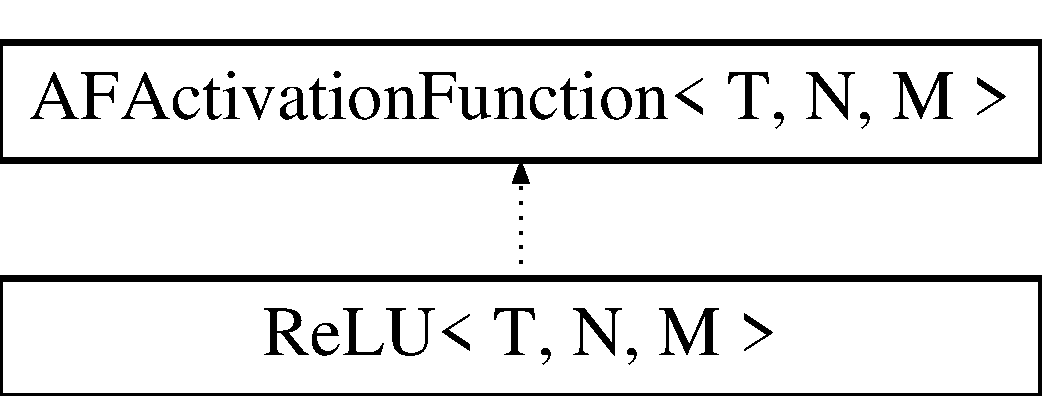
\includegraphics[height=2.000000cm]{class_re_l_u}
\end{center}
\end{figure}


The documentation for this class was generated from the following file\+:\begin{DoxyCompactItemize}
\item 
C\+:/\+Users/\+Aryan/\+C\+Lion\+Projects/\+C\+Net/src/\hyperlink{_a_f_activation_function_8h}{A\+F\+Activation\+Function.\+h}\end{DoxyCompactItemize}

\chapter{File Documentation}
\hypertarget{_a_f_activation_function_8cpp}{}\section{C\+:/\+Users/\+Aryan/\+C\+Lion\+Projects/\+C\+Net/src/\+A\+F\+Activation\+Function.cpp File Reference}
\label{_a_f_activation_function_8cpp}\index{C\+:/\+Users/\+Aryan/\+C\+Lion\+Projects/\+C\+Net/src/\+A\+F\+Activation\+Function.\+cpp@{C\+:/\+Users/\+Aryan/\+C\+Lion\+Projects/\+C\+Net/src/\+A\+F\+Activation\+Function.\+cpp}}
{\ttfamily \#include \char`\"{}A\+F\+Activation\+Function.\+h\char`\"{}}\newline

\hypertarget{_a_f_activation_function_8h}{}\section{C\+:/\+Users/\+Aryan/\+C\+Lion\+Projects/\+C\+Net/src/\+A\+F\+Activation\+Function.h File Reference}
\label{_a_f_activation_function_8h}\index{C\+:/\+Users/\+Aryan/\+C\+Lion\+Projects/\+C\+Net/src/\+A\+F\+Activation\+Function.\+h@{C\+:/\+Users/\+Aryan/\+C\+Lion\+Projects/\+C\+Net/src/\+A\+F\+Activation\+Function.\+h}}
{\ttfamily \#include $<$vector$>$}\newline
{\ttfamily \#include $<$math.\+h$>$}\newline
\subsection*{Classes}
\begin{DoxyCompactItemize}
\item 
class \hyperlink{class_a_f_activation_function}{A\+F\+Activation\+Function}
\item 
class \hyperlink{class_re_l_u}{Re\+LU}
\end{DoxyCompactItemize}

\hypertarget{_a_f_matrix_8cpp}{}\section{src/\+A\+F\+Matrix.cpp File Reference}
\label{_a_f_matrix_8cpp}\index{src/\+A\+F\+Matrix.\+cpp@{src/\+A\+F\+Matrix.\+cpp}}
{\ttfamily \#include \char`\"{}A\+F\+Matrix.\+h\char`\"{}}\newline

\hypertarget{_a_f_matrix_8h}{}\section{C\+:/\+Users/\+Aryan/\+C\+Lion\+Projects/\+C\+Net/src/\+A\+F\+Matrix.h File Reference}
\label{_a_f_matrix_8h}\index{C\+:/\+Users/\+Aryan/\+C\+Lion\+Projects/\+C\+Net/src/\+A\+F\+Matrix.\+h@{C\+:/\+Users/\+Aryan/\+C\+Lion\+Projects/\+C\+Net/src/\+A\+F\+Matrix.\+h}}
{\ttfamily \#include $<$array$>$}\newline
\subsection*{Classes}
\begin{DoxyCompactItemize}
\item 
class \hyperlink{class_a_f_matrix}{A\+F\+Matrix$<$ T, R\+O\+W\+S, C\+O\+L\+S $>$}
\end{DoxyCompactItemize}
\subsection*{Functions}
\begin{DoxyCompactItemize}
\item 
{\footnotesize template$<$typename T , size\+\_\+t N$>$ }\\T \hyperlink{_a_f_matrix_8h_aab0242d9abf78560470c22023ee5d701}{vector\+Inner\+Product} (array$<$ T, N $>$ $\ast$vec1, array$<$ T, N $>$ $\ast$vec2)
\item 
{\footnotesize template$<$typename T , size\+\_\+t N$>$ }\\T \hyperlink{_a_f_matrix_8h_a3642605226af032c63df0ec34ae85cf6}{vector\+Inner\+Product} (array$<$ T, N $>$ $\ast$vec1, array$<$ T, N $>$ $\ast$vec2, int start1, int end1, int start2, int end2)
\end{DoxyCompactItemize}


\subsection{Function Documentation}
\mbox{\Hypertarget{_a_f_matrix_8h_aab0242d9abf78560470c22023ee5d701}\label{_a_f_matrix_8h_aab0242d9abf78560470c22023ee5d701}} 
\index{A\+F\+Matrix.\+h@{A\+F\+Matrix.\+h}!vector\+Inner\+Product@{vector\+Inner\+Product}}
\index{vector\+Inner\+Product@{vector\+Inner\+Product}!A\+F\+Matrix.\+h@{A\+F\+Matrix.\+h}}
\subsubsection{\texorpdfstring{vector\+Inner\+Product()}{vectorInnerProduct()}\hspace{0.1cm}{\footnotesize\ttfamily [1/2]}}
{\footnotesize\ttfamily template$<$typename T , size\+\_\+t N$>$ \\
T vector\+Inner\+Product (\begin{DoxyParamCaption}\item[{array$<$ T, N $>$ $\ast$}]{vec1,  }\item[{array$<$ T, N $>$ $\ast$}]{vec2 }\end{DoxyParamCaption})\hspace{0.3cm}{\ttfamily [inline]}}


\begin{DoxyTemplParams}{Template Parameters}
{\em T} & The type of data in the vectors being multiplies. Probably a {\ttfamily double}. \\
\hline
\end{DoxyTemplParams}

\begin{DoxyParams}{Parameters}
{\em vec1} & -\/ Left vector \\
\hline
{\em vec2} & -\/ Right vector \\
\hline
\end{DoxyParams}
\begin{DoxyReturn}{Returns}
The dot product (inner product) of two vectors. 
\end{DoxyReturn}
\begin{DoxyPrecond}{Precondition}
vec1 and vec2 have the same length. 
\end{DoxyPrecond}
\mbox{\Hypertarget{_a_f_matrix_8h_a3642605226af032c63df0ec34ae85cf6}\label{_a_f_matrix_8h_a3642605226af032c63df0ec34ae85cf6}} 
\index{A\+F\+Matrix.\+h@{A\+F\+Matrix.\+h}!vector\+Inner\+Product@{vector\+Inner\+Product}}
\index{vector\+Inner\+Product@{vector\+Inner\+Product}!A\+F\+Matrix.\+h@{A\+F\+Matrix.\+h}}
\subsubsection{\texorpdfstring{vector\+Inner\+Product()}{vectorInnerProduct()}\hspace{0.1cm}{\footnotesize\ttfamily [2/2]}}
{\footnotesize\ttfamily template$<$typename T , size\+\_\+t N$>$ \\
T vector\+Inner\+Product (\begin{DoxyParamCaption}\item[{array$<$ T, N $>$ $\ast$}]{vec1,  }\item[{array$<$ T, N $>$ $\ast$}]{vec2,  }\item[{int}]{start1,  }\item[{int}]{end1,  }\item[{int}]{start2,  }\item[{int}]{end2 }\end{DoxyParamCaption})}


\begin{DoxyTemplParams}{Template Parameters}
{\em T} & The type of data in the vectors being multiplies. Probably a {\ttfamily double}. \\
\hline
\end{DoxyTemplParams}

\begin{DoxyParams}{Parameters}
{\em vec1} & -\/ Left vector \\
\hline
{\em vec2} & -\/ Right vector \\
\hline
\end{DoxyParams}
\begin{DoxyReturn}{Returns}
The dot product (inner product) of two vectors. 
\end{DoxyReturn}
\begin{DoxyPrecond}{Precondition}
vec1 and vec2 have the same length. 
\end{DoxyPrecond}

\hypertarget{_layer_8cpp}{}\section{C\+:/\+Users/\+Aryan/\+C\+Lion\+Projects/\+C\+Net/src/\+Layer.cpp File Reference}
\label{_layer_8cpp}\index{C\+:/\+Users/\+Aryan/\+C\+Lion\+Projects/\+C\+Net/src/\+Layer.\+cpp@{C\+:/\+Users/\+Aryan/\+C\+Lion\+Projects/\+C\+Net/src/\+Layer.\+cpp}}
{\ttfamily \#include \char`\"{}Layer.\+h\char`\"{}}\newline

\hypertarget{_layer_8h}{}\section{C\+:/\+Users/\+Aryan/\+C\+Lion\+Projects/\+C\+Net/src/\+Layer.h File Reference}
\label{_layer_8h}\index{C\+:/\+Users/\+Aryan/\+C\+Lion\+Projects/\+C\+Net/src/\+Layer.\+h@{C\+:/\+Users/\+Aryan/\+C\+Lion\+Projects/\+C\+Net/src/\+Layer.\+h}}
{\ttfamily \#include \char`\"{}A\+F\+Activation\+Function.\+h\char`\"{}}\newline
{\ttfamily \#include \char`\"{}A\+F\+Matrix.\+h\char`\"{}}\newline
{\ttfamily \#include $<$iostream$>$}\newline
\subsection*{Classes}
\begin{DoxyCompactItemize}
\item 
class \hyperlink{class_layer}{Layer$<$ L\+E\+N\+\_\+\+I\+N, L\+E\+N\+\_\+\+O\+U\+T $>$}
\end{DoxyCompactItemize}

\hypertarget{main_8cpp}{}\section{C\+:/\+Users/\+Aryan/\+C\+Lion\+Projects/\+C\+Net/src/main.cpp File Reference}
\label{main_8cpp}\index{C\+:/\+Users/\+Aryan/\+C\+Lion\+Projects/\+C\+Net/src/main.\+cpp@{C\+:/\+Users/\+Aryan/\+C\+Lion\+Projects/\+C\+Net/src/main.\+cpp}}
{\ttfamily \#include $<$iostream$>$}\newline
\subsection*{Functions}
\begin{DoxyCompactItemize}
\item 
int \hyperlink{main_8cpp_ae66f6b31b5ad750f1fe042a706a4e3d4}{main} ()
\end{DoxyCompactItemize}


\subsection{Function Documentation}
\mbox{\Hypertarget{main_8cpp_ae66f6b31b5ad750f1fe042a706a4e3d4}\label{main_8cpp_ae66f6b31b5ad750f1fe042a706a4e3d4}} 
\index{main.\+cpp@{main.\+cpp}!main@{main}}
\index{main@{main}!main.\+cpp@{main.\+cpp}}
\subsubsection{\texorpdfstring{main()}{main()}}
{\footnotesize\ttfamily int main (\begin{DoxyParamCaption}{ }\end{DoxyParamCaption})}


\hypertarget{_net_8cpp}{}\section{src/\+Net.cpp File Reference}
\label{_net_8cpp}\index{src/\+Net.\+cpp@{src/\+Net.\+cpp}}
{\ttfamily \#include \char`\"{}Net.\+h\char`\"{}}\newline

\hypertarget{_net_8h}{}\section{src/\+Net.h File Reference}
\label{_net_8h}\index{src/\+Net.\+h@{src/\+Net.\+h}}
\subsection*{Classes}
\begin{DoxyCompactItemize}
\item 
class \hyperlink{class_net}{Net$<$ T $>$}
\end{DoxyCompactItemize}

%--- End generated contents ---

% Index
\backmatter
\newpage
\phantomsection
\clearemptydoublepage
\addcontentsline{toc}{chapter}{Index}
\printindex

\end{document}
